% Options for packages loaded elsewhere
\PassOptionsToPackage{unicode}{hyperref}
\PassOptionsToPackage{hyphens}{url}
\PassOptionsToPackage{dvipsnames,svgnames*,x11names*}{xcolor}
%
\documentclass[
]{krantz}
\usepackage{lmodern}
\usepackage{amssymb,amsmath}
\usepackage{ifxetex,ifluatex}
\ifnum 0\ifxetex 1\fi\ifluatex 1\fi=0 % if pdftex
  \usepackage[T1]{fontenc}
  \usepackage[utf8]{inputenc}
  \usepackage{textcomp} % provide euro and other symbols
\else % if luatex or xetex
  \usepackage{unicode-math}
  \defaultfontfeatures{Scale=MatchLowercase}
  \defaultfontfeatures[\rmfamily]{Ligatures=TeX,Scale=1}
\fi
% Use upquote if available, for straight quotes in verbatim environments
\IfFileExists{upquote.sty}{\usepackage{upquote}}{}
\IfFileExists{microtype.sty}{% use microtype if available
  \usepackage[]{microtype}
  \UseMicrotypeSet[protrusion]{basicmath} % disable protrusion for tt fonts
}{}
\makeatletter
\@ifundefined{KOMAClassName}{% if non-KOMA class
  \IfFileExists{parskip.sty}{%
    \usepackage{parskip}
  }{% else
    \setlength{\parindent}{0pt}
    \setlength{\parskip}{6pt plus 2pt minus 1pt}}
}{% if KOMA class
  \KOMAoptions{parskip=half}}
\makeatother
\usepackage{xcolor}
\IfFileExists{xurl.sty}{\usepackage{xurl}}{} % add URL line breaks if available
\IfFileExists{bookmark.sty}{\usepackage{bookmark}}{\usepackage{hyperref}}
\hypersetup{
  pdftitle={Multimodal Deep Learning},
  colorlinks=true,
  linkcolor=Maroon,
  filecolor=Maroon,
  citecolor=Blue,
  urlcolor=Blue,
  pdfcreator={LaTeX via pandoc}}
\urlstyle{same} % disable monospaced font for URLs
\usepackage{longtable,booktabs}
% Correct order of tables after \paragraph or \subparagraph
\usepackage{etoolbox}
\makeatletter
\patchcmd\longtable{\par}{\if@noskipsec\mbox{}\fi\par}{}{}
\makeatother
% Allow footnotes in longtable head/foot
\IfFileExists{footnotehyper.sty}{\usepackage{footnotehyper}}{\usepackage{footnote}}
\makesavenoteenv{longtable}
\usepackage{graphicx,grffile}
\makeatletter
\def\maxwidth{\ifdim\Gin@nat@width>\linewidth\linewidth\else\Gin@nat@width\fi}
\def\maxheight{\ifdim\Gin@nat@height>\textheight\textheight\else\Gin@nat@height\fi}
\makeatother
% Scale images if necessary, so that they will not overflow the page
% margins by default, and it is still possible to overwrite the defaults
% using explicit options in \includegraphics[width, height, ...]{}
\setkeys{Gin}{width=\maxwidth,height=\maxheight,keepaspectratio}
% Set default figure placement to htbp
\makeatletter
\def\fps@figure{htbp}
\makeatother
\setlength{\emergencystretch}{3em} % prevent overfull lines
\providecommand{\tightlist}{%
  \setlength{\itemsep}{0pt}\setlength{\parskip}{0pt}}
\setcounter{secnumdepth}{5}
\usepackage{booktabs}
\usepackage{longtable}
\usepackage[bf,singlelinecheck=off]{caption}

\usepackage{framed,color}
\definecolor{shadecolor}{RGB}{248,248,248}

\renewcommand{\textfraction}{0.05}
\renewcommand{\topfraction}{0.8}
\renewcommand{\bottomfraction}{0.8}
\renewcommand{\floatpagefraction}{0.75}

\renewenvironment{quote}{\begin{VF}}{\end{VF}}
\let\oldhref\href
\renewcommand{\href}[2]{#2\footnote{\url{#1}}}

\makeatletter
\newenvironment{kframe}{%
\medskip{}
\setlength{\fboxsep}{.8em}
 \def\at@end@of@kframe{}%
 \ifinner\ifhmode%
  \def\at@end@of@kframe{\end{minipage}}%
  \begin{minipage}{\columnwidth}%
 \fi\fi%
 \def\FrameCommand##1{\hskip\@totalleftmargin \hskip-\fboxsep
 \colorbox{shadecolor}{##1}\hskip-\fboxsep
     % There is no \\@totalrightmargin, so:
     \hskip-\linewidth \hskip-\@totalleftmargin \hskip\columnwidth}%
 \MakeFramed {\advance\hsize-\width
   \@totalleftmargin\z@ \linewidth\hsize
   \@setminipage}}%
 {\par\unskip\endMakeFramed%
 \at@end@of@kframe}
\makeatother

\usepackage{makeidx}
\makeindex

\urlstyle{tt}

\usepackage{amsthm}
\makeatletter
\def\thm@space@setup{%
  \thm@preskip=8pt plus 2pt minus 4pt
  \thm@postskip=\thm@preskip
}
\makeatother

\frontmatter
\usepackage[]{natbib}
\bibliographystyle{apalike}

\title{Multimodal Deep Learning}
\author{}
\date{\vspace{-2.5em}2022-03-29}

\begin{document}
\maketitle

% you may need to leave a few empty pages before the dedication page

%\cleardoublepage\newpage\thispagestyle{empty}\null
%\cleardoublepage\newpage\thispagestyle{empty}\null
%\cleardoublepage\newpage
\thispagestyle{empty}

\begin{center}
\end{center}

\setlength{\abovedisplayskip}{-5pt}
\setlength{\abovedisplayshortskip}{-5pt}

{
\hypersetup{linkcolor=}
\setcounter{tocdepth}{0}
\tableofcontents
}
\hypertarget{preface}{%
\chapter*{Preface}\label{preface}}


\begin{figure}
\centering

\includegraphics{figures/by-nc-sa.png}
\caption{Creative Commons License}
\end{figure}

This book is licensed under the \href{http://creativecommons.org/licenses/by-nc-sa/4.0/}{Creative Commons Attribution-NonCommercial-ShareAlike 4.0 International License}.

\mainmatter

\hypertarget{foreword}{%
\chapter*{Foreword}\label{foreword}}


\emph{Author: Christoph Molnar}

This book is the result of an experiment in university teaching.
Each semester, students of the Statistics Master can choose from a selection of seminar topics.
Usually, every student in the seminar chooses a scientific paper, gives a talk about the paper and summarizes it in the form of a seminar paper.
The supervisors help the students, they listen to the talks, read the seminar papers, grade the work and then \ldots{} hide the seminar papers away in (digital) drawers.
This seemed wasteful to us, given the huge amount of effort the students usually invest in seminars.
An idea was born:
Why not create a book with a website as the outcome of the seminar?
Something that will last at least a few years after the end of the semester.
In the summer term 2019, some Statistics Master students signed up for our seminar entitled ``Limitations of Interpretable Machine Learning''.
When they came to the kick-off meeting, they had no idea that they would write a book by the end of the semester.

We were bound by the examination rules for conducting the seminar, but otherwise we could deviate from the traditional format.
We deviated in several ways:

\begin{enumerate}
\def\labelenumi{\arabic{enumi}.}
\tightlist
\item
  Each student project is part of a book, and not an isolated seminar paper.
\item
  We gave challenges to the students, instead of papers. The challenge was to investigate a specific limitation of interpretable machine learning methods.
\item
  We designed the work to live beyond the seminar.
\item
  We emphasized collaboration. Students wrote some chapters in teams and reviewed each others texts.
\end{enumerate}

\hypertarget{technical-setup}{%
\section*{Technical Setup}\label{technical-setup}}


The book chapters are written in the Markdown language.
The simulations, data examples and visualizations were created with R \citep{rlang}.
To combine R-code and Markdown, we used rmarkdown.
The book was compiled with the bookdown package.
We collaborated using git and github.
For details, head over to the \href{https://github.com/slds-lmu/seminar_multimodal_dl}{book's repository}.

\hypertarget{introduction}{%
\chapter{Introduction}\label{introduction}}

\emph{Author: }

\emph{Supervisor: }

\hypertarget{intro-about-the-seminar-topic}{%
\section{Intro About the Seminar Topic}\label{intro-about-the-seminar-topic}}

\hypertarget{outline-of-the-booklet}{%
\section{Outline of the Booklet}\label{outline-of-the-booklet}}

\hypertarget{introducing-the-modalities}{%
\chapter{Introducing the modalities}\label{introducing-the-modalities}}

\emph{Author: }

\emph{Supervisor: }

\hypertarget{title}{%
\chapter{title}\label{title}}

\emph{Author: }

\emph{Supervisor: }

\hypertarget{title-1}{%
\chapter{title}\label{title-1}}

\emph{Author: }

\emph{Supervisor: }

\hypertarget{chapter-1}{%
\chapter{Chapter 1}\label{chapter-1}}

\emph{Authors: Author 1, Author 2}

\emph{Supervisor: Supervisor}

\hypertarget{lorem-ipsum}{%
\section{Lorem Ipsum}\label{lorem-ipsum}}

Lorem ipsum dolor sit amet, consetetur sadipscing elitr, sed diam nonumy eirmod tempor invidunt ut labore et dolore magna aliquyam erat, sed diam voluptua. At vero eos et accusam et justo duo dolores et ea rebum. Stet clita kasd gubergren, no sea takimata sanctus est Lorem ipsum dolor sit amet. Lorem ipsum dolor sit amet, consetetur sadipscing elitr, sed diam nonumy eirmod tempor invidunt ut labore et dolore magna aliquyam erat, sed diam voluptua. At vero eos et accusam et justo duo dolores et ea rebum. Stet clita kasd gubergren, no sea takimata sanctus est Lorem ipsum dolor sit amet.

\citet{rlang}

\hypertarget{using-figures}{%
\section{Using Figures}\label{using-figures}}

\begin{figure}

{\centering 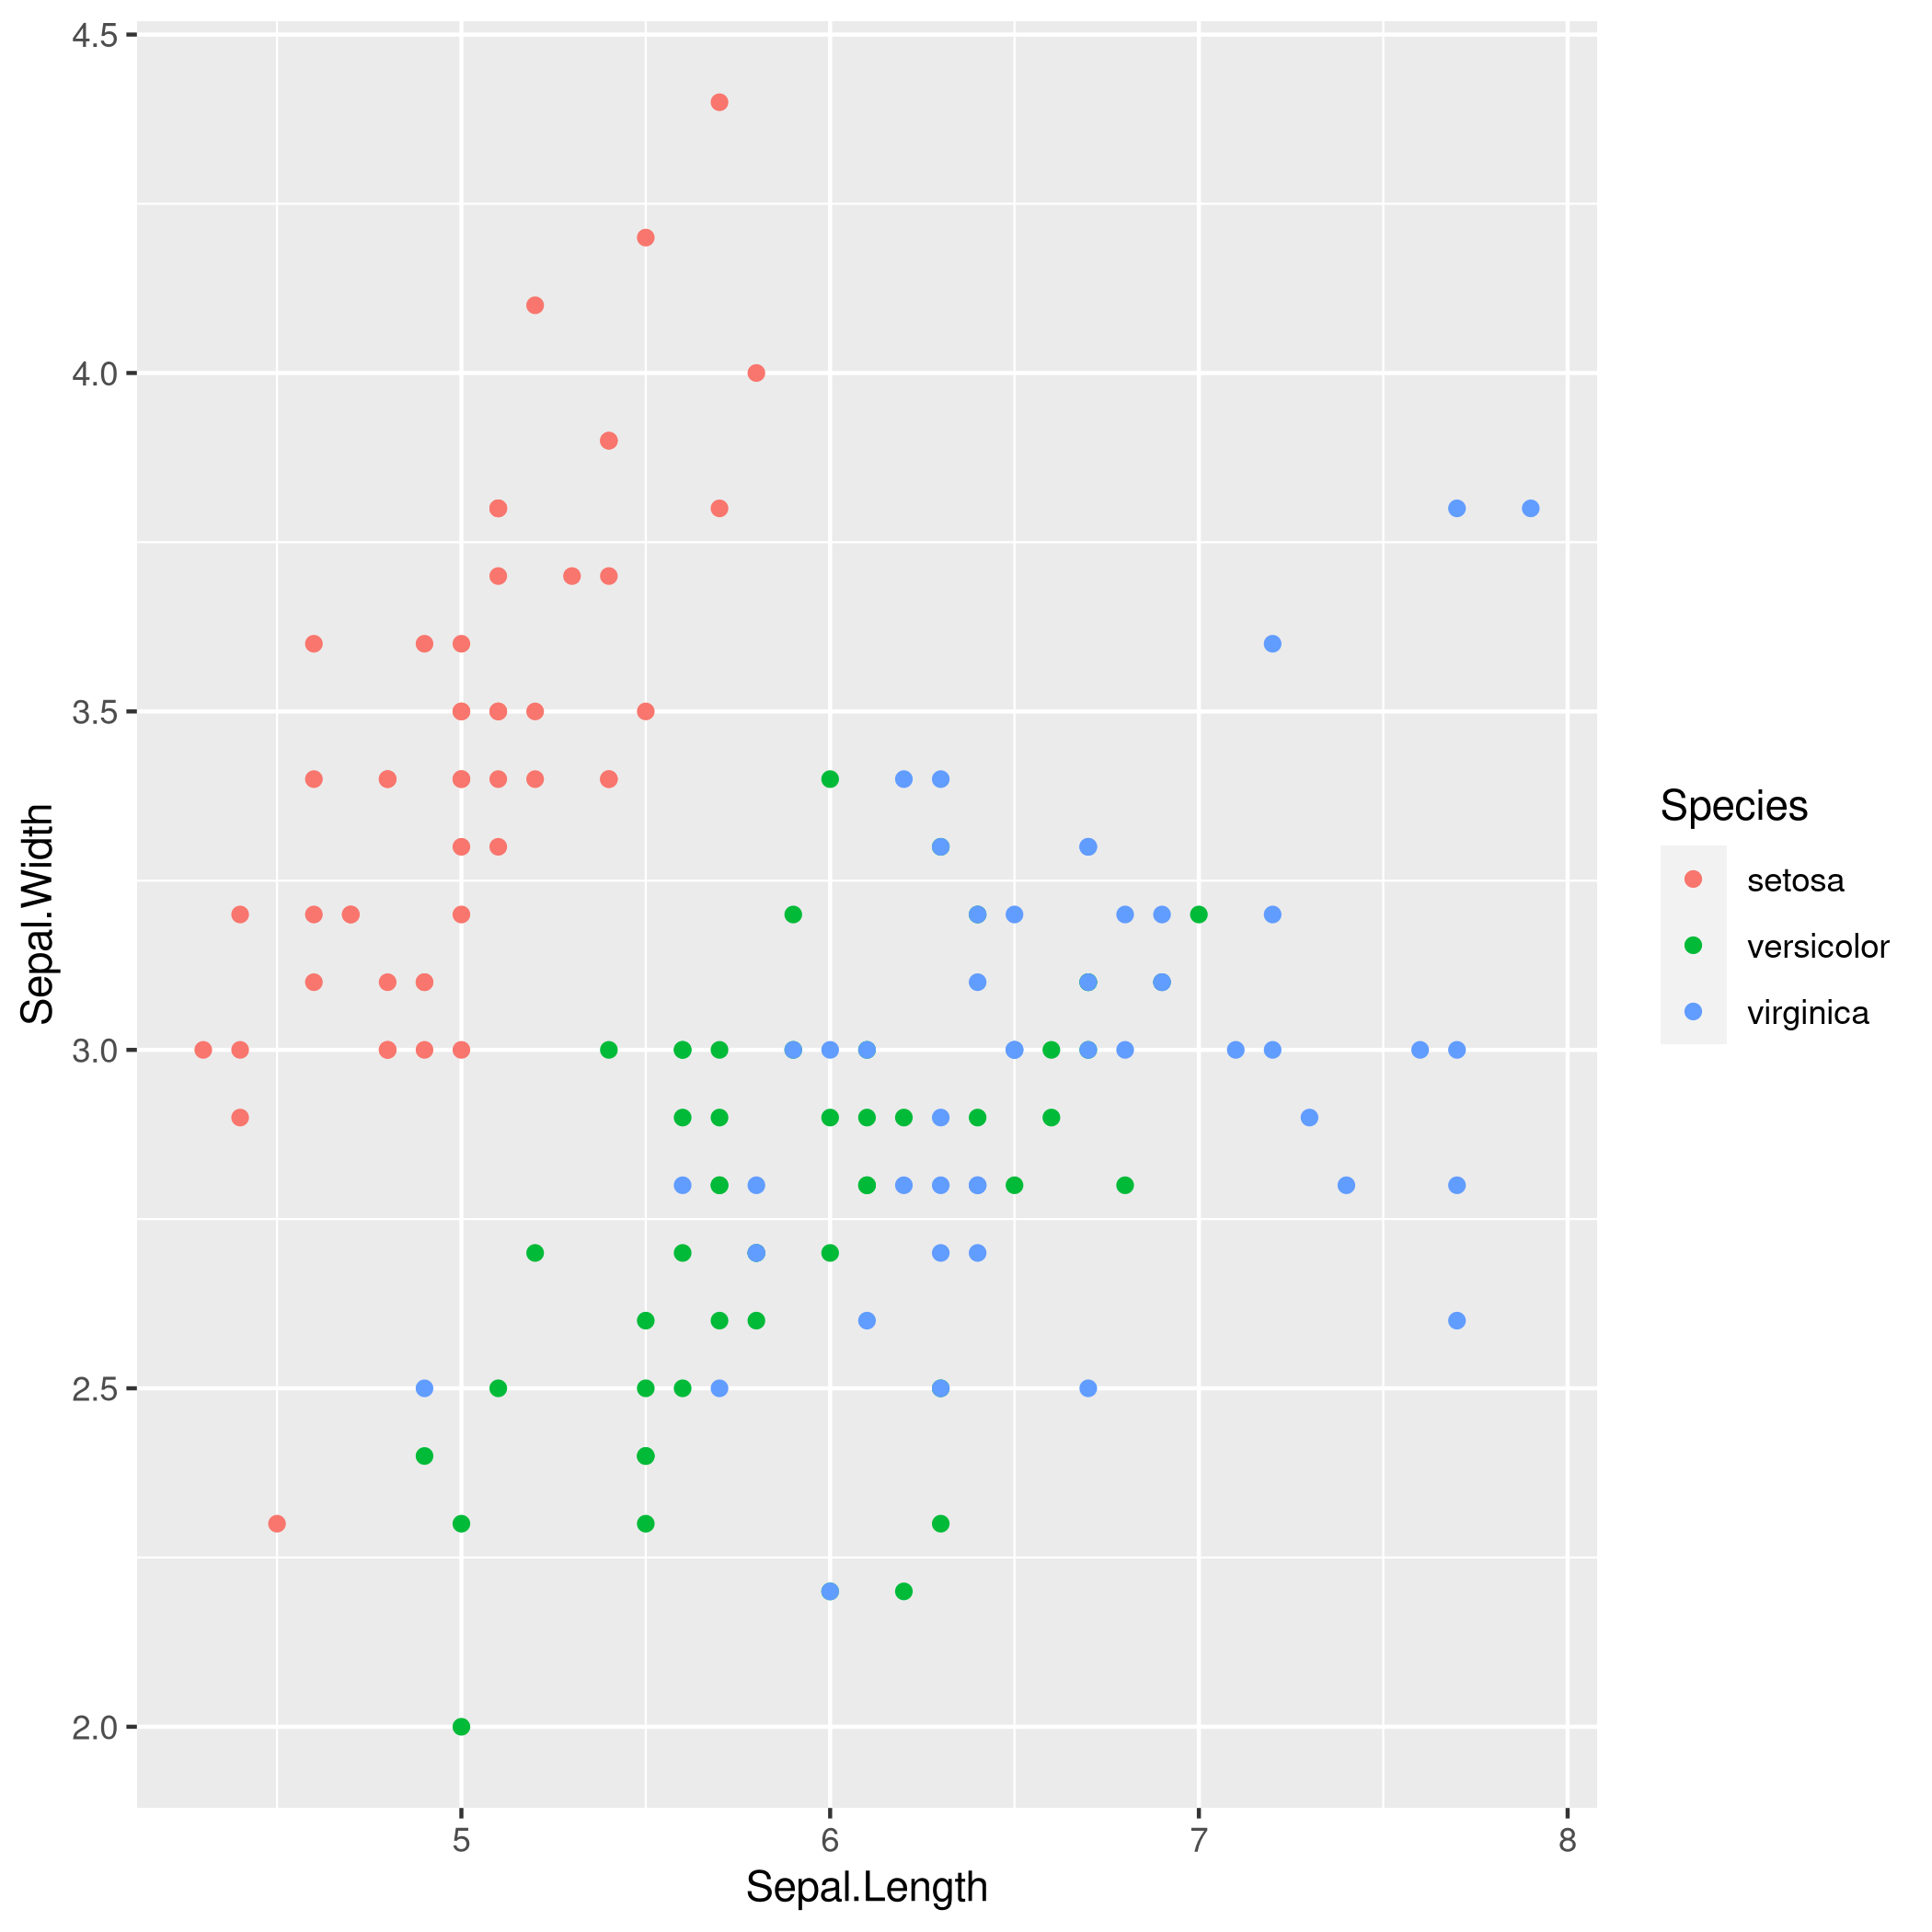
\includegraphics[width=0.8\linewidth]{figures/01-chapter1/ch01-figure01} 

}

\caption{This is the caption of the figure!}\label{fig:ch01-figure01}
\end{figure}



Referencing can be done by using the chunk label e.g.~\texttt{\textbackslash{}@ref(fig:ch01-figure01)} for \ref{fig:ch01-figure01}.

\textbf{NOTE!!!} Do not use underscores in chunk labels! This will crash the compilation \ldots{}

\hypertarget{using-tex}{%
\section{Using Tex}\label{using-tex}}

HTML rendering uses MathJax while pdf rendering uses LaTeX:

\[
f(x) = x^2
\]

\hypertarget{using-stored-results}{%
\section{Using Stored Results}\label{using-stored-results}}

\begin{tabular}{l|r|r|r|r}
\hline
  & Estimate & Std. Error & t value & Pr(>|t|)\\
\hline
(Intercept) & 2.1713 & 0.2798 & 7.760 & 0.0000\\
\hline
Sepal.Width & 0.4959 & 0.0861 & 5.761 & 0.0000\\
\hline
Petal.Length & 0.8292 & 0.0685 & 12.101 & 0.0000\\
\hline
Petal.Width & -0.3152 & 0.1512 & -2.084 & 0.0389\\
\hline
Speciesversicolor & -0.7236 & 0.2402 & -3.013 & 0.0031\\
\hline
Speciesvirginica & -1.0235 & 0.3337 & -3.067 & 0.0026\\
\hline
\end{tabular}

\hypertarget{chapter-2}{%
\chapter{Chapter 2}\label{chapter-2}}

\emph{Authors: Author 1, Author 2}

\emph{Supervisor: Supervisor}

\hypertarget{lorem-ipsum-1}{%
\section{Lorem Ipsum}\label{lorem-ipsum-1}}

Lorem ipsum dolor sit amet, consetetur sadipscing elitr, sed diam nonumy eirmod tempor invidunt ut labore et dolore magna aliquyam erat, sed diam voluptua. At vero eos et accusam et justo duo dolores et ea rebum. Stet clita kasd gubergren, no sea takimata sanctus est Lorem ipsum dolor sit amet. Lorem ipsum dolor sit amet, consetetur sadipscing elitr, sed diam nonumy eirmod tempor invidunt ut labore et dolore magna aliquyam erat, sed diam voluptua. At vero eos et accusam et justo duo dolores et ea rebum. Stet clita kasd gubergren, no sea takimata sanctus est Lorem ipsum dolor sit amet.

\citet{rlang}

\hypertarget{epilogue}{%
\chapter{Epilogue}\label{epilogue}}

\emph{Author: }

\hypertarget{test}{%
\section{test}\label{test}}

\hypertarget{acknowledgements}{%
\chapter{Acknowledgements}\label{acknowledgements}}

The most important contributions are from the students themselves.
The success of such projects highly depends on the students.
And this book is a success, so thanks a lot to all the authors!
The other important role is the supervisor.
Thanks to all the supervisors who participated!
Special thanks to \href{https://www.misoda.statistik.uni-muenchen.de/personen/professoren/heumann/index.html}{Christian Heumann} and \href{https://www.statistik.uni-muenchen.de/personen/professoren/bischl/index.html}{Bernd Bischl} who enabled us to conduct the seminar in such an experimental way, supported us and gave valuable feedback for the seminar structure.
Thanks a lot as well to the entire \href{https://www.statistik.uni-muenchen.de/}{Department of Statistics} and the \href{http://www.en.uni-muenchen.de/index.html}{LMU Munich} for the infrastructure.

The authors of this work take full responsibilities for its content.

  \bibliography{book.bib,packages.bib}

\backmatter
\printindex

\end{document}
